\documentclass{article}

% Packages
\usepackage{fancyhdr}
\usepackage{extramarks}
\usepackage{amsmath}
\usepackage{amsthm}
\usepackage{amsfonts}
\usepackage{tikz}
\usepackage[plain]{algorithm}
\usepackage{algpseudocode}
\usepackage{enumerate}

\usetikzlibrary{automata,positioning}

% Document Layout
\topmargin=-0.45in
\evensidemargin=0in
\oddsidemargin=0in
\textwidth=6.5in
\textheight=9.0in
\headsep=0.25in
\linespread{1.1}

% Page Style
\pagestyle{fancy}
\lhead{\hmwkAuthorName}
\chead{\hmwkClass:\ \hmwkTitle}
\rhead{Section \hmwkSection, \firstxmark}
\lfoot{\lastxmark}
\cfoot{\thepage}
\renewcommand\headrulewidth{0.4pt}
\renewcommand\footrulewidth{0.4pt}

% Paragraph Settings
\setlength\parindent{0pt}
\setlength{\parskip}{5pt}

% Section Management
\newcommand{\hmwkSection}{A} % Current section (A, B, or C) - update manually

% Problem Header Management
\newcommand{\enterProblemHeader}[1]{
  \nobreak\extramarks{}{Problem \arabic{#1} continued on next page\ldots}\nobreak{}
  \nobreak\extramarks{Problem \arabic{#1} (continued)}{Problem \arabic{#1} continued on next page\ldots}\nobreak{}
}

\newcommand{\exitProblemHeader}[1]{
  \nobreak\extramarks{Problem \arabic{#1} (continued)}{Problem \arabic{#1} continued on next page\ldots}\nobreak{}
  \stepcounter{#1}
  \nobreak\extramarks{Problem \arabic{#1}}{}\nobreak{}
}

% Counters
\setcounter{secnumdepth}{0}
\newcounter{partCounter}
\newcounter{homeworkProblemCounter}
\setcounter{homeworkProblemCounter}{1}
\nobreak\extramarks{Problem \arabic{homeworkProblemCounter}}{}\nobreak{}

% Homework Problem Environment
% Optional argument adjusts problem counter for non-sequential problems
\newenvironment{homeworkProblem}[1][-1]{
  \ifnum#1>0
    \setcounter{homeworkProblemCounter}{#1}
  \fi
  \section{Problem \arabic{homeworkProblemCounter}}
  \setcounter{partCounter}{1}
  \enterProblemHeader{homeworkProblemCounter}
}{
  \exitProblemHeader{homeworkProblemCounter}
}

% Assignment Details
\newcommand{\hmwkTitle}{Sheet\ \#1}
\newcommand{\hmwkDueDate}{October 22, 2025}
\newcommand{\hmwkClass}{SC9 Probability on Graphs and Lattices}
\newcommand{\hmwkClassInstructor}{Professor C. Goldschmidt and Professor J. Jorritsma}
\newcommand{\hmwkAuthorName}{\textbf{Ray Tsai}}

% Title Page
\title{
  \vspace{2in}
  \textmd{\textbf{\hmwkClass:\ \hmwkTitle}}\\
  \normalsize\vspace{0.1in}\small{Due\ on\ \hmwkDueDate\ at 12:00pm}\\
  \vspace{0.1in}\large{\textit{\hmwkClassInstructor}} \\
  \vspace{3in}
}

\author{\hmwkAuthorName}
\date{}

% Part Command
\renewcommand{\part}[1]{\textbf{\large Part \Alph{partCounter}}\stepcounter{partCounter}\\}

% Mathematical Commands
% Algorithms
\newcommand{\alg}[1]{\textsc{\bfseries \footnotesize #1}}

% Calculus
\newcommand{\deriv}[1]{\frac{\mathrm{d}}{\mathrm{d}x} (#1)}
\newcommand{\pderiv}[2]{\frac{\partial}{\partial #1} (#2)}
\newcommand{\dx}{\mathrm{d}x}

% Probability and Statistics
\newcommand{\Var}{\mathrm{Var}}
\newcommand{\Cov}{\mathrm{Cov}}
\newcommand{\Bias}{\mathrm{Bias}}
\newcommand*{\prob}{\mathbb{P}}
\newcommand*{\E}{\mathbb{E}}

% Number Sets
\newcommand*{\Z}{\mathbb{Z}}
\newcommand*{\Q}{\mathbb{Q}}
\newcommand*{\R}{\mathbb{R}}
\newcommand*{\C}{\mathbb{C}}
\newcommand*{\N}{\mathbb{N}}

\begin{document}

\maketitle
\pagebreak

\begin{homeworkProblem}
  Given a finite, connected graph $G$, and a path of neighbouring vertices $(x_0, x_1, x_2, \dots)$ such that every vertex $v \in V(G)$ appears in the path, let $\tau_v := \inf\{n : x_n = v\}$. Let $T$ be the subgraph of $G$ with $V(T) = V(G)$ and edge-set
  \[
    E(T) := \{\{x_{\tau_v-1}, x_{\tau_v}\} : v \in V(G) \setminus \{x_0\}\}.
  \]
  Prove that $T$ is a spanning tree for $G$.
\end{homeworkProblem}

\newpage

\begin{homeworkProblem}
  \begin{enumerate}[(a)]
    \item Consider the \textit{coupon collector's problem}: boxes of a certain cereal come with one of $n$ distinct coupons, chosen uniformly at random, and you wish to collect the full set of $n$ coupons.
    Show that the expected number $N_n$ of boxes of cereal that you have to buy is such that
    \[
      \E[N_n] \sim n \log n
    \]
    as $n \to \infty$.
    \item Use (a) to give an upper bound on the expected number of steps taken by the Aldous-Broder algorithm on the complete graph $K_n$.
  \end{enumerate}
\end{homeworkProblem}

\newpage

\begin{homeworkProblem}
  Consider the graph $G$:

  \begin{center}
  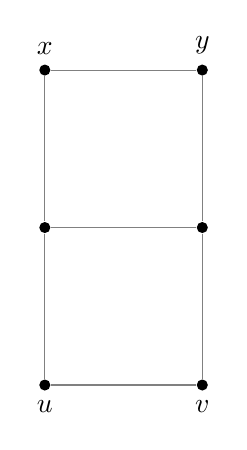
\begin{tikzpicture}
    % --- Define a style for the nodes ---
    % 'dot' style: a solid black circle, 2pt radius
    \tikzset{
      dot/.style = {circle, fill=black, inner sep=0pt, minimum size=4pt}
    }
    
    % --- Place the nodes ---
    % We use (x,y) coordinates to position them in a grid.
    % We also give each node a name, e.g., (x), (u), (m1).
    \node[dot, label=above:$x$] (x)  at (0, 4) {};
    \node[dot, label=above:$y$] (y)  at (2, 4) {};
    \node[dot]                 (m1) at (0, 2) {};
    \node[dot]                 (m2) at (2, 2) {};
    \node[dot, label=below:$u$] (u)  at (0, 0) {};
    \node[dot, label=below:$v$] (v)  at (2, 0) {};
    
    % --- Draw the edges ---
    % Connect the nodes using their names.
    % We can chain commands to draw the vertical lines efficiently.
    \draw [gray] (x) -- (y);  % Top edge
    \draw [gray] (m1) -- (m2); % Middle edge
    \draw [gray] (u) -- (v);  % Bottom edge
    
    \draw [gray] (x) -- (m1) -- (u); % Left vertical edges
    \draw [gray] (y) -- (m2) -- (v); % Right vertical edges
    
  \end{tikzpicture}
  \end{center}
    
  Let $e = \{u, v\}$ and $e' = \{x, y\}$. Let $T$ be a UST of $G$. Show that $\prob_u^G(\tau_v < \tau_u^+) = 15/22$ and $\prob_u^{G/e'}(\tau_v < \tau_u^+) = 11/16$. Deduce that, in this case, we indeed have
  \[
    \prob(e \in E(T) | e' \in E(T)) \le \prob(e \in E(T)).
  \]
  \textit{This question is partly intended as a reminder of how to do hitting probability calculations! You may find it helpful in each case to write down a system of simultaneous equations and solve them (using a computer if you like) to find the desired probabilities.}
\end{homeworkProblem}

\newpage

\begin{homeworkProblem}
  For every vertex $v_i \in V(G) \setminus \{v_0\}$, select a directed edge $\vec{v_i w_i}$. Prove that this collection of directed edges is either a spanning tree on $G$ directed towards $v_0$, or includes a directed cycle.
\end{homeworkProblem}

\newpage

\renewcommand{\hmwkSection}{B}

\begin{homeworkProblem}
  By reference to Wilson's algorithm, or otherwise, prove that in a finite or recurrent connected graph $G$, the law of the loop-erased random walk path from $x$ to $y$ is the same as the law of the loop-erased random walk path from $y$ to $x$.
    
  \textit{Note: the loop-erased random walk path from $x$ to $y$ is constructed by taking the (almost surely finite) path of a random walk from $x$ stopped at $\tau_y$, and then loop-erasing it.}

  \begin{proof}
    Since $G$ is connected and recurrent, we may generate FUSF on $G$ using Wilson's algorithm. For $v \in V(G)$, let $T_v$ be a random variable for the FUSF on $G$ generated by Wilson's algorithm by setting $v_0 = v$. By Proposition 1.19, $T_v$ is a.s. connected. Thus there exists a path a.s. from any $u \in V(G) \backslash \{v\}$ to $v$, denoted $P_v(u)$, and we note that $P_v(u)$ is a LERW. Since the distribution of the generated FUSF is independent of the root, $\mu_{T_v}$ is the same for any $v \in V(G)$. Let $A \subset E(G)$ denote a collection of edges that forms a path between $x$ and $y$. SInce $\mu_{T_x} = \mu_{T_y}$, 
    \[
      \prob(P_x(y) = A) = \prob(A \subset E(T_x)) = \prob(A \subset E(T_y)) = \prob(P_y(x) = A).
    \]
    This completes the proof.
  \end{proof}
\end{homeworkProblem}

\newpage

\begin{homeworkProblem}
  Let $T_n$ be a UST of the complete graph $K_n$. Let $v, w, w'$ be distinct vertices in $K_n$ and consider edges $e = \{v, w\}$ and $e' = \{v, w'\}$. Use the Aldous-Broder algorithm to prove that $e, e'$ are negatively associated in $T_n$ i.e. that
  \[
    \prob(e, e' \in E(T_n)) \le \prob(e \in E(T_n)) \prob(e' \in E(T_n))
  \]
  for all sufficiently large $n$.

  \begin{proof}
    Consider the Aldous-Broder algorithm starting from $v$. Let $A$ be the event that $e \in E(T_n)$ and $B$ be the event that $e' \in E(T_n)$. Let $X_i$ denote the $i$-th step of the SRW from $v$. Note that $e \in E(T_n)$ if and only if $e$ is the first entry into $w$. That is, either it happnes immediately, or requires the SRW to return to $v$ before reaching $w$. Thus by the Strong Markov Property,
    \[
      \prob(A) = \frac{1}{n - 1} + \prob_v(\tau_v^+ < \tau_w)\prob(A),
    \]
    where $\prob_v$ denotes the probability measure on the SRW starting from $v$. Since $\prob_v(\tau_v^+ = \tau_w) = 0$, rearranging the above equation yields
    \[
      \prob(A) = \frac{1}{(n - 1)\prob(\tau_v^+ > \tau_w)}.
    \]
    Note that
    \begin{align*}
      \prob_v(\tau_v^+ > \tau_w) 
      &= \prob_v(\tau_v^+ > \tau_w \mid X_1 = w)\prob_v(X_1 = w) + \sum_{u \in V(G) \backslash e} \prob_v(\tau_v^+ > \tau_w \mid X_1 = u)\prob_v(X_1 = u) \\
      &= \frac{1}{n - 1} + \frac{1}{n - 1}\sum_{u \in V(G) \backslash e} \prob_u(\tau_v > \tau_w).
    \end{align*}
    By symmetry, $\prob_u(\tau_v > \tau_w) = \prob_u(\tau_w > \tau_v)$, so $\prob_u(\tau_v > \tau_w) = 1/2$. Hence, we have
    \[
      \prob_v(\tau_v^+ > \tau_w) = \frac{1}{n - 1} + \frac{n - 2}{n - 1} \cdot\frac{1}{2} = \frac{n}{2(n - 1)},
    \]
    and thus $\prob(A) = 2/n$. By symmetry, $\prob(B) = 2/n$. 

    We now compute $\prob(A \cap B)$. We may write
    \[
      \prob(A \cap B) = \frac{1}{n - 1} \cdot \sum_{u \in V(G) \backslash \{v\}} \prob(A \cap B \mid X_1 = u)
    \]
    If $X_1 = w$, then by the same symmetry argument,
    \[
      \prob(A \cap B \mid X_1 = w) = \prob(B | X_1 = w) = \prob_w(\tau_v < \tau_{w'})P(B) = \frac{1}{2} \cdot \frac{2}{n} = \frac{1}{n}.
    \]
    Similarly, we also have $\prob(A \cap B \mid X_1 = w') = \frac{1}{n}$. Now suppose $X_1 = u$ for some $u \in V(G)\backslash \{v, w, w'\}$. Then,
    \[
      \prob(A \cap B \mid X_1 = u) = \prob_u(\tau_{v} < \tau_w \text{ and } \tau_{v} < \tau_{w'}) \prob(A \cap B) = \frac{1}{3} \cdot \prob(A \cap B),
    \]
    as the probability of first reaching either $v, w, $ or $w'$ is the same. Substituting back to the initial equation,
    \[
      \prob(A \cap B) = \frac{1}{n - 1}\left(\frac{2}{n} + (n - 3) \cdot \frac{1}{3} \cdot \prob(A \cap B)\right).
    \]
    Rearranging yields 
    \[
      \prob(A \cap B) = \frac{3}{n^2} \leq \frac{4}{n^2} = \prob(A)\prob(B).
    \]
    This completes the proof.
  \end{proof}
\end{homeworkProblem}

\newpage

\begin{homeworkProblem}
  Prove that the free uniform spanning forest on an infinite, connected, locally-finite graph $G$ has no finite components almost surely.

  \begin{proof}
    Let $(G_n)$ be some exhaustion of $G$, with associated USTs $(T_n)$. Let $F$ be a FUSF of $G$. Let $C \subset V(G)$ be a finite set of vertices, and define
    \[
      \mathcal{K}_C = \{\{u, v\} \in E(G) : u \in C, v \in V(G)\backslash C\}.
    \] 
    Since $G$ is conencted and locally finite, $\mathcal{K}_C$ is nonempty and finite. Let $E_C$ be the event that $C$ is a component in $F$. Then $E_C$ implies the cylinder event $A_C = \{E(F) \cap \mathcal{K}_C = \emptyset\}$, so $\prob(E_C) \leq \prob(A_C)$. We now show that $\prob(A_C) = 0$. Note that 
    \[
      \prob(A_C) = \mu^F(A_C) = \lim_{n \to \infty}\mu_{T_n}(A_C) = \lim_{n \to \infty} \prob(E(T_n) \cap \mathcal{K}_C = \emptyset).
    \]
    Suppose $n$ is large enough such that $C$ is strictly contained in $V(G_n)$. Since $G_n$ is connected and $T_n$ is a spanning tree, $T_n$ must contain a path from $C$ to $V(G_n)\backslash C$. That is, $T_n$ must contain some edge in $G$. But then
    \[
      \prob(A_C) = \lim_{n \to \infty} \prob(E(T_n) \cap \mathcal{K}_C = \emptyset) = 0.
    \]
    It now follows that
    \[
      \prob(F \text{ has some finite component}) = \prob\left(\bigcup_{\substack{C \subset V(G) \\ |C| < \infty}} E_C\right) \leq \sum_{\substack{C \subset V(G) \\ |C| < \infty}} \prob(E_C) \leq \sum_{\substack{C \subset V(G) \\ |C| < \infty}} \prob(A_C) = 0.
    \]
  \end{proof}
\end{homeworkProblem}

\newpage

\begin{homeworkProblem}
  Let $G$ be the lattice $\Z^2$. Given the box $G_n = [-n, n]^2 \cap \Z^2$, the Dobrushin wiring $G_n^{\text{Dob}}$ consists of adding a vertex $u_n$, and an edge between $u_n$ and each of the $4n+2$ vertices which lie either on the left-boundary or the right-boundary. Let $T_n^{\text{Dob}}$ be the UST on $G_n^{\text{Dob}}$, and let $\mu_{G_n^{\text{Dob}}}$ be the probability measure on $\Omega_G$ describing the restriction of $T_n^{\text{Dob}}$ to $G_n \subset G$. Prove that $\mu_{G_n^{\text{Dob}}} \Rightarrow \mu^F$.

  \begin{proof}
    Let $A \subset E(G)$ be some finite set of edges, and let $\mathcal{C}_A = \{\omega \in \Omega_G : w(e) = 1, \, \forall e \in A\}$. Since $\mathcal{C}_A$ is an increasing cylinder event, by Proposition 1.17, it suffices to show that 
    \[
      \lim_{n \to \infty} \mu_{G^{\text{Dob}}_n}(\mathcal{C}_A) = \mu^F(\mathcal{C}_A).
    \]
    Assume $n$ large enough such that $A \subset E(G_n)$. Consider the wired subgraph $(G_n^W)$ and the associated USTs $(T_n^W)$. Notice that $G_n \subseteq G_n^{\text{Dob}} \subseteq G_n^W$, so
    \[
      \mu_{T_n^W}(\mathcal{C}_A) \leq \mu_{G_n^{\text{Dob}}}(\mathcal{C}_A) \leq \mu_{T_n}(\mathcal{C}_A).
    \]
    But then $G$ is recurrent and connected, so by Proposition 1.26,
    \[
      \lim_{n \to \infty} \mu_{T_n^W}(\mathcal{C}_A) = \lim_{n \to \infty} \mu_{T_n}(\mathcal{C}_A) = \mu^F(\mathcal{C}_A).
    \]
    The desired result now follows from sandwiching.
  \end{proof}
\end{homeworkProblem}

\newpage

\begin{homeworkProblem}
  Let $G$ be an infinite, recurrent, connected graph with an exhaustion $(G_n)$. By coupling a random walk on $G$ and a random walk on $G_n$ appropriately, show that the Aldous-Broder algorithm also generates the UST on $G$ (which you should view as the FUSF on $G$, defined along an exhaustion).

  \begin{proof}
    Let $(T_n)$ be the associated USTs of $(G_n)$. Let $A \subset E(G)$ be finite, with $\mathcal{C}_A$ the corresponding cylinder event. Let $\mathcal{A} \subset V(G)$ denote the finite set of vertices incident to $A$. Assume that $n$ is large enough that $\mathcal{A} \subset V_n$. 

    Now run Aldous-Broder algorithm on $G$. Since $G$ is recurrent and connected, the SRW will hit every vertex in $\mathcal{A}$. Note that we can also run Aldous-Broder algorithm on $G_n$ using the same SRW, and the partial subtrees generated will be the same until the SRW hits $\partial G_n$. But then the restrictions of $T$ and $T_n$ to $\mathcal{A}$ are different only if the SRW hit $\partial G_n$ before hitting every vertex in $\mathcal{A}$. Let $\tau_{\partial G}$ denote the hitting time of $\partial G$ and we have
    \begin{align*}
      |\prob(A \subset E(T)) - \prob(A \subset E(T_n))| 
      &\leq \prob(\{A \subset E(T)\} \Delta \{A \subset E(T_n)\}) \\
      &\leq \prob(T \text{ restricted to } \mathcal{A} \text{ not built before }\tau_{\partial G_n}) \\
      &\leq \prob\left(\bigcup_{v \in \mathcal{A}} \{\tau_v > \tau_{\partial G_n}\}\right) \\
      &\leq \sum_{v \in \mathcal{A}} \prob(\tau_v > \tau_{\partial G_n}),
    \end{align*}
    by the union bound. Since $G$ is recurrent, $\prob(\tau_v > \tau_{\partial G_n}) \to 0$ as $n \to \infty$. Thus we have
    \[
      \lim_{n \to \infty} \prob(A \subset E(T_n)) = \prob(A \subset E(T)).
    \]
    The result now follows from Proposition 1.17.
  \end{proof}
\end{homeworkProblem}

\newpage

\renewcommand{\hmwkSection}{C}

\begin{homeworkProblem}[10]
  Consider again the coupon collector's problem from Question 2. For $k \ge 0$ let $C_n(k)$ be the number of coupons which have not yet been collected by step $k$, so that $C_n(0) = n$ and $C_n(1) = n-1$.
  \begin{enumerate}[(a)]
    \item Let $M_n(k) = \left(1 - \frac{1}{n}\right)^{-k} C_n(k)$. Show that $\E[M_n(k+1) | C_n(k)] = M_n(k)$ (i.e. the process $(M_n(k))_{k \ge 0}$ is a martingale).
    \item Hence show that $\prob(N_n > \lceil n \log n + cn \rceil) \le e^{-c}$ for any $c > 0$.
  \end{enumerate}
\end{homeworkProblem}

\newpage

\begin{homeworkProblem}[11]
  Let $G = (V, E)$ be a connected recurrent graph, and let $(X_n)_{n > 0}$ be a simple random walk on $G$, which moves around on the vertices of the graph, at each step independently moving to a neighbour of its current position chosen uniformly at random.
  \begin{enumerate}[(a)]
    \item For a fixed directed edge $(v, w)$, find the mean return time to $(v, w)$.
    \item Deduce the edge-commute identity:
    $$ \E_v[\tau_w] + \E_w[\tau_v] \le 2|E|, $$
    where $\tau_u := \inf\{n \ge 0 : X_n = u\}$ for $u \in V$.
    \item Let $t_{\text{cov}}$ be the cover time of $G$, that is the first time that the SRW has visited all the vertices. Prove that for any spanning tree $t$ of $G$ and any vertex $u \in V$ we have
    $$ \E_u[t_{\text{cov}}] \le \sum_{\{v,w\} \in t} (\E_v[\tau_w] + \E_w[\tau_v]), $$
    and deduce an upper bound on $\max_{u \in V} \E_u[t_{\text{cov}}]$ in terms of $|E|$.
    \item Further deduce that the expected number of steps in the Aldous-Broder algorithm is bounded above by $|V|^3$ for any graph.
    \item Give an example of a graph for which the upper bound in (c) is of the correct order and an example of a graph for which it is not.
  \end{enumerate}
\end{homeworkProblem}

\newpage

\begin{homeworkProblem}[12]
  On the complete graph $K_n$, with $n \ge 2$, Aldous (1990) gave another algorithm to generate a UST, as follows.
  Let $U_2, \dots, U_n$ be uniform on $\{1, 2, \dots, n-1\}$. Start from a single vertex labelled 1.
  \begin{itemize}
      \item For $2 \le i \le n$ connect vertex $i$ to vertex $V_i = \min\{U_i, i-1\}$.
      \item Relabel vertices $1, \dots, n$ as $\pi(1), \dots, \pi(n)$ where $\pi$ is a uniform random permutation of $1, \dots, n$.
  \end{itemize}
  (Note that this algorithm has only $n-1$ steps, and so is considerably more efficient than Aldous-Broder on $K_n$!)
  \begin{enumerate}[(a)]
    \item Starting from the Aldous-Broder algorithm, or otherwise, verify that this algorithm indeed yields a UST of $K_n$.
    \item Let $L_n^{(1)}$ be the first index at which $\min\{U_i, i-1\} \ne i-1$. Find $\prob(L_n^{(1)} \ge k+1)$.
    \item Show that $L_n^{(1)} / \sqrt{n} \to L^{(1)}$ where $L^{(1)}$ has density $f(x) = x e^{-x^2/2}$, $x \ge 0$.
    \item Now let $L_n^{(2)}$, $L_n^{(3)}, \dots$ be the successive subsequent indices at which $\min\{U_i, i-1\} \ne i-1$. What can you say about the joint limit in distribution of
    $$ \frac{1}{\sqrt{n}} (L_n^{(1)}, L_n^{(2)} - L_n^{(1)}, \dots, L_n^{(m)} - L_n^{(m-1)}) $$
    for $m \ge 2$ as $n \to \infty$?
  \end{enumerate}
  This shows that the correct "length-scale" for the UST on $K_n$ is $\sqrt{n}$. Indeed, much more is true: the result above is an important aspect of the convergence of the UST on $K_n$, on rescaling by $1/\sqrt{n}$ to the so-called Brownian continuum random tree.
\end{homeworkProblem}

\newpage

\begin{homeworkProblem}[13]
  Let $T$ be the UST on $\Z^2$, and let $S_n$ be the subgraph of $T$ induced on the box $\Lambda_n = [-n, n]^2 \cap \Z^2$.
  \begin{enumerate}[(a)]
    \item Find the best constants $\alpha_n$, $\beta_n$ such that
    \[
      \alpha_n \le |E(S_n)| \le \beta_n
    \]
    holds almost surely.
    Hint: you may find it helpful to consider the connectivity of the wired version of $S_n$.
    \item Hence, or otherwise, show that if $e$ is any edge of $\Z^2$ then
    \[
      \prob(e \in E(T)) = \frac{1}{2}.
    \]
  \end{enumerate}
\end{homeworkProblem}

\newpage

\begin{homeworkProblem}[14]
  Let $T$ be the UST on $\Z^2$.
  \begin{enumerate}[(a)]
      \item Show that there exist two adjacent vertices on the boundary of the box $[-n, n]^2 \cap \Z^2$ that are connected by a path in $T$ with length at least $2n$.
      \item Let $L$ be the length of the path from $(0,0)$ to $(0,1)$ in $T$. Use (a) to show that
      \[
        \prob(L \ge 2n) \ge \frac{1}{8n}.
      \]
  \end{enumerate}
\end{homeworkProblem}

\end{document}